% RankMixer Paper Review Summary (LaTeX)
\documentclass{article}
\usepackage[margin=1in]{geometry}
\usepackage{graphicx}
\usepackage[T1]{fontenc}
\begin{document}

\section*{RankMixer: Scaling Up Ranking Models in Industrial Recommenders (2025)}
\textbf{arXiv:2507.15551v3 (cs.IR), 26 Jul 2025.}

\subsection*{Challenges}
\begin{itemize}
  \item \textbf{CPU-era feature-crossing modules fail to exploit modern GPUs:} low MFU (4–5\%) and poor parallelism hinder scaling in production ranking.
  \item \textbf{Strict latency and QPS constraints:} industrial recommender systems must serve high QPS under tight latency budgets, limiting naive parameter scaling.
  \item \textbf{Imbalanced expert training in Sparse-MoE:} dynamic routing and load imbalance can starve experts and degrade performance at scale.
\end{itemize}

\subsection*{Key Initiatives}
\begin{itemize}
  \item \textbf{Hardware-aware feature interaction (TokenMixer):} replace self-attention with a multi-head token mixing module for GPU-friendly parallel cross‑feature fusion.
  \item \textbf{Per-token FFNs for subspace modeling:} allocate separate FFNs per token to capture distinct feature subspaces and avoid parameter sharing bottlenecks.
  \item \textbf{Sparse-MoE extension for 1B+ scale:} integrate dynamic routing (DTSI-ReLU) to scale to 1B parameters with minimal latency impact and balanced expert training.
  \item \textbf{Unified transformer-like blocks:} ranker architecture with residual connections + LayerNorm + TokenMixer + PFFN blocks achieves high MFU and compute efficiency.
\end{itemize}

\subsection*{Methodology}
\begin{itemize}
  \item \textbf{RankMixer block (Figure~\ref{fig:arch}):} each block applies a Multi-Head Token Mixing layer followed by a Per-Token Feed-Forward Network, both wrapped in residual + LayerNorm.
  \item \textbf{Sparse-MoE variant:} activate a subset of per-token FFNs via dynamic routing, boosting capacity 70× with only a 20× FLOPs increase (MFU soared 4.5\%→44.6\%).
  \item \textbf{Scaling directions:} width (D), token count (T), and layers (L) can be scaled orthogonally following Transformer-like scaling laws.
\end{itemize}

\begin{figure}[h]
  \centering
  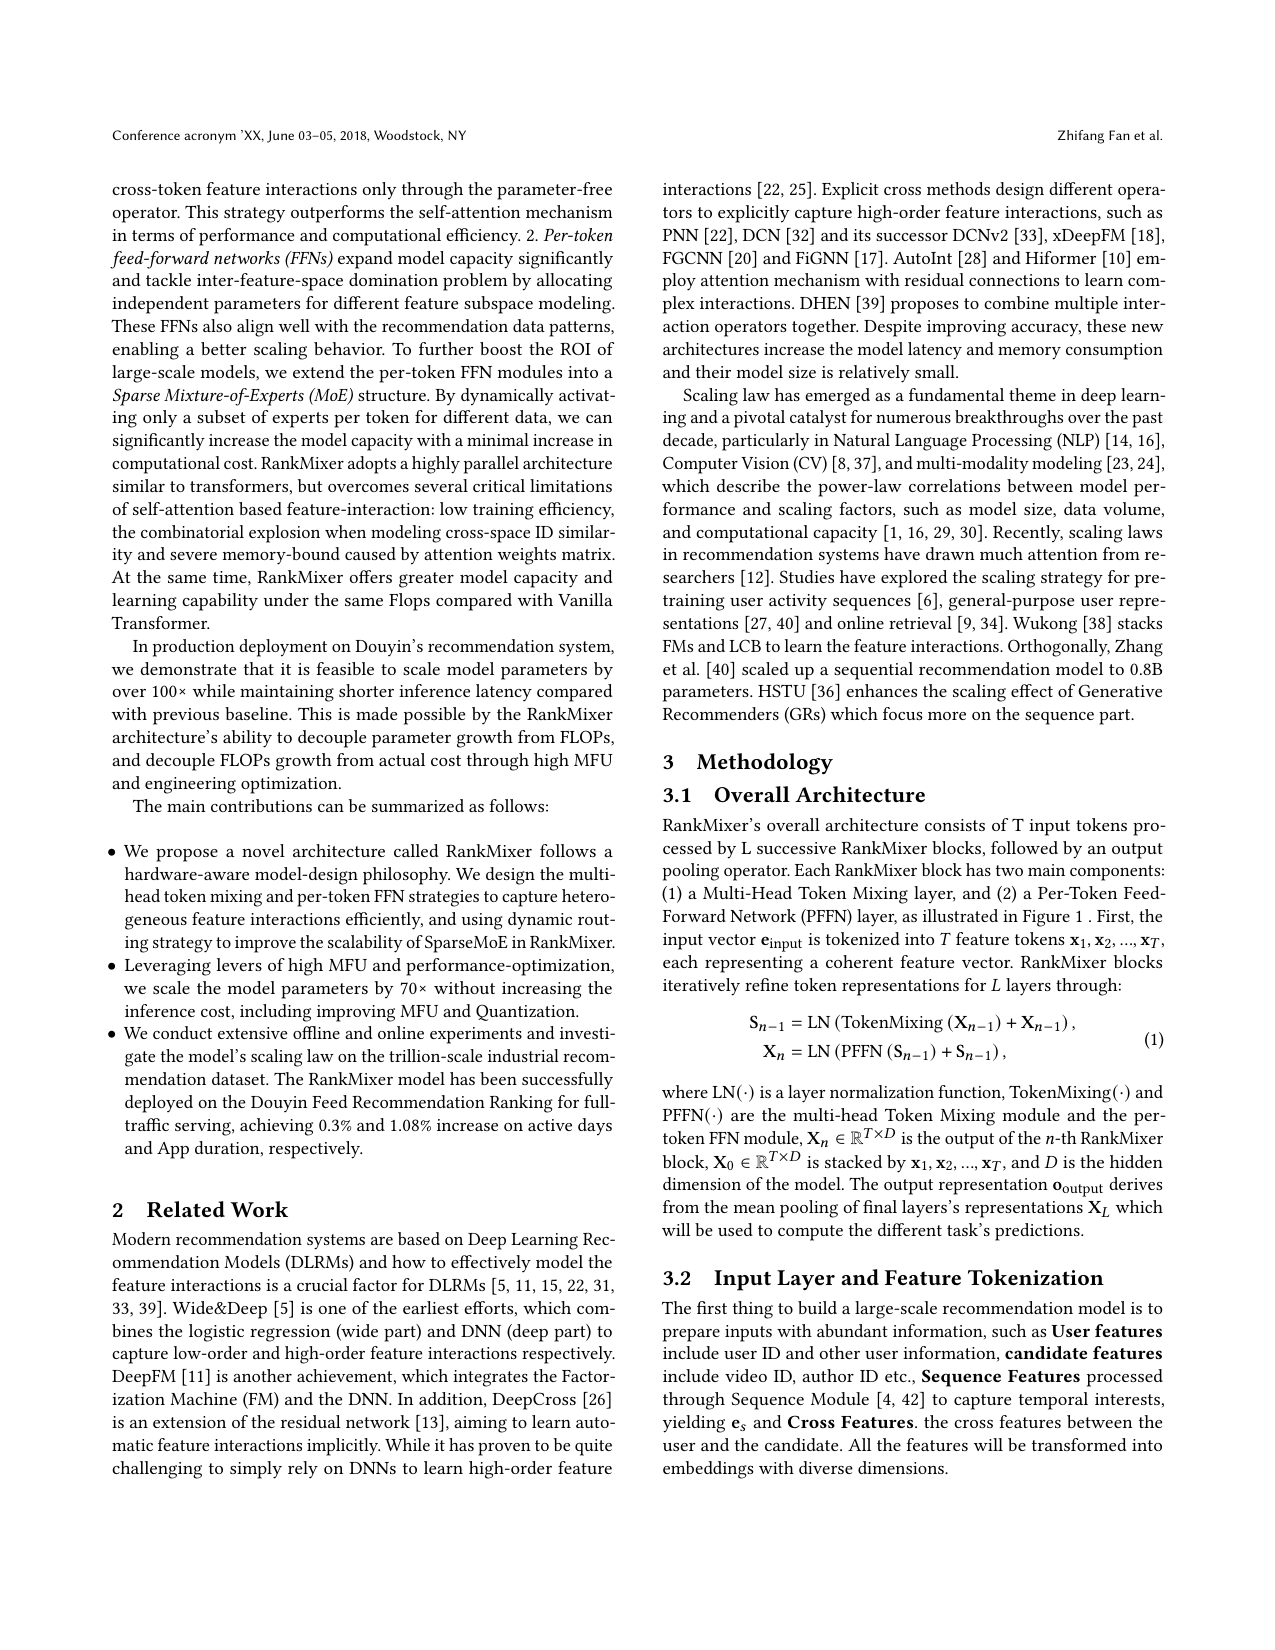
\includegraphics[width=\linewidth]{fig1_rankmixer_block.png}
  \caption{Architecture of a RankMixer block (Figure 1).}
  \label{fig:arch}
\end{figure}

\subsection*{Experiments}
\begin{itemize}
  \item \textbf{Offline performance/efficiency (Table 1):} RankMixer-100M outperforms SOTA cross-structure models (+0.64\% AUC / +0.72\% UAUC) with 233G FLOPs vs baselines at up to 442G.
  \item \textbf{Component ablations (Tables 2 \& 3):} Multi-Head Token Mixing and per-token FFNs are critical (–0.50\%/–0.31\% AUC w/o);
  \item \textbf{Online A/B lift (Tables 4–6):} 1B model improved feed active days +0.29\%, app duration +1.08\%; advertising AUC +0.73\%, revenue +3.90\%. MFU ↑10×, latency flat.
  \item \textbf{Scalability \& expert balance (Figures~2--4):} dynamic Sparse-MoE retains accuracy under 1/8 activation ratio; consistent scaling laws across Params/FLOPs.
\end{itemize}

\subsection*{References (selected)}
\begin{itemize}
  \item Transformer scaling laws: Hoffmann et al., 2022; Kaplan et al., 2020.
  \item Sparse Mixture-of-Experts routing: Lepikhin et al., 2020; Shazeer et al., 2017.
  \item Cross-feature interaction: Guo et al., 2017 (DeepFM); Tang et al., 2019 (DCNv2); Luan et al., 2023 (CrossFormer).
  \item Modern scaling in RecSys: Zhang et al., 2024 (Wukong); Zhai et al., 2025 (HSTU); Rajput et al., 2023 (TIGER).
\end{itemize}

\end{document}
